\cotefile{109}
\scanpage{2}
\begin{center}\uline{Notations}\end{center}
\diagram{%
\(\begin{array}{@{}l@{\quad}l@{\quad}l@{}}
\mathord{\tikz[x=1ex,y=1ex,baseline=0pt]{\draw (0,0)--(0,1.45)--(1.35,1.45)--(1.35,0) (.19,0)--(.19,1.45);}}_{n}(X) & ?\ \text{\deleted{\illegible{1}}} & \\[3pt]
{}^{\unsure{1|4}}\overset{i}{\underset{\ell}{*}},\,\check{u}
  & ?\ \text{\deleted{\illegible{1}}} & \\[3pt]
(\mathrm{Cat})\ \begin{array}[c]{l}
 \inserted{(\unsure{\mathrm{Ss}|\mathrm{ss}}\text{-}\mathrm{sets})\quad16}\\[-2pt]
 \deleted{(\mathrm{ss}\text{-}\mathrm{sets})\unsure{\simeq|=}\mathord{\tikz[x=1ex,y=1ex,baseline=0pt]{\draw (0,0)--(.96,1.35)--(1.48,0)--cycle (.19,0)--(1.02,1.17);}}^{\unsure{\wedge|?}}\quad16}
 \end{array}
 & \multicolumn{2}{l}{\mathord{\tikz[x=1ex,y=1ex,baseline=0pt]{\draw (0,0)--(.96,1.35)--(1.48,0)--cycle (.19,0)--(1.02,1.17);}}\qquad \mathord{\tikz[x=1ex,y=1ex,baseline=0pt]{\draw (0,0) rectangle (1.38,1.26) (.19,0)--(.19,1.26);}}\qquad \mathord{\tikz[x=1ex,y=1ex,baseline=0pt]{\draw (0.65,0.65) ellipse (.61 and .72) (.76,1.35) .. controls (.13,1.04) and (.19,.30) .. (.73,-.05);}}}\\[3pt]
\multicolumn{3}{l}{A_{/\unsure{x|X}},\,A^{\circ},\, A^{\wedge}\ \text{ou}\ \hat A}\\[3pt]
\begin{array}[t]{@{}l|} K\unsure{\text{---}|\longrightarrow|\mapsto}|K|\\
(\mathrm{Ord})\\
(\mathrm{Preord})\\
\deleted{\unsure{\mathcal C|C}^{\circ}}\ (\mathrm{Hot})\\
\inserted{\Delta_n}\mathord{\tikz[baseline=0pt,overlay]{\draw (-.35em,-.2ex)--(.55em,2.5ex);}}\ \mathord{\tikz[x=1ex,y=1ex,baseline=0pt]{\draw (0,0)--(.96,1.35)--(1.48,0)--cycle (.19,0)--(1.02,1.17);}},\,\mathord{\tikz[x=1ex,y=1ex,baseline=0pt]{\draw (0,0)--(.96,1.35)--(1.48,0)--cycle (.19,0)--(1.02,1.17);}}[N]
\end{array}
 & 22 & \\[3pt]
\begin{array}{@{}l|} \mathord{\tikz[x=1ex,y=1ex,baseline=0pt]{\draw (0,0) rectangle (1.38,1.26) (.19,0)--(.19,1.26);}},\,\mathord{\tikz[x=1ex,y=1ex,baseline=0pt]{\draw (0,0) rectangle (1.38,1.26) (.19,0)--(.19,1.26);}}_{n}\end{array}
 & \unsure{24|29} & \\[3pt]
\widetilde{\mathord{\tikz[x=1ex,y=1ex,baseline=0pt]{\draw (0,0) rectangle (1.38,1.26) (.19,0)--(.19,1.26);}}}\quad\widetilde{\mathord{\tikz[x=1ex,y=1ex,baseline=0pt]{\draw (0,0)--(.96,1.35)--(1.48,0)--cycle (.19,0)--(1.02,1.17);}}} &34&
\end{array}\)}
\clearpage
% archive sheet number: 1
\scanpage{3}
\uline{Introduction}

chiffres soulignés \unsure{dans|ds|des} table des matières. \hfill / signe $[\,\ldots\,]$

Modifications \unsure{mineures|numérotées} dans lettre à \ldots

Stacks $=$ non \unsure{commutative} chain complexes (cf. p.~4)
\clearpage
% archive sheet number: 2
\scanpage{4}
\begin{center}\uline{Imprimeur}\end{center}
\diagram{\begin{tikzcd}[ampersand replacement=\&,column sep=2.4em,row sep=.5em]
\underline{N} \arrow[r,mapsto] \& \mathbb{N}\\
\unsure{\not{1}|\not{l}|\not{\ell}} \arrow[r,mapsto] \& \ell
\end{tikzcd}}
\figure{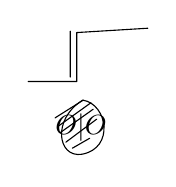
\begin{tikzpicture}[x=.55cm,y=.55cm,line cap=round,line join=round]
\draw (0,0)--(1.12,0)--(1.12,1.13)--(2.76,1.23) (0.97,.10)--(.97,1.16);
\node[inner sep=0pt] at (1.22,-1.07) {$\deleted{\unsure{\mathbb{O}|O}}$};
\draw (1.26,-.43) .. controls (1.83,-.52) and (2.00,-1.54) .. (1.24,-1.68)
 .. controls (.68,-1.77) and (.54,-.87) .. (1.26,-.43);
\draw (.62,-.84)--(1.27,-.43) (.71,-1.02)--(1.45,-.49)
 (.74,-1.18)--(1.50,-.64) (.87,-1.40)--(1.58,-.87)
 (1.02,-1.54)--(1.42,-1.31);
\end{tikzpicture}}
% paper watermark, running down the sheet
\begin{center}\tikz{\node[rotate=-90]{EXTRA STRONG};}\end{center}
\clearpage
% archive sheet number: 3
\scanpage{5}
Index des notations

\[
\begin{aligned}
&\overset{\approx}{\longrightarrow} &&\overset{\sim}{\longrightarrow}\\
&\approx &&\simeq
\end{aligned}
\]

\[
\tikz[baseline=(z.base)]{\node[draw,circle,inner sep=2pt] (z) {$\underline{Z}$};}
\quad\mathbb{R}\quad\mathbb{Q}\quad\mathbb{C}
\]

\[
\mathord{\tikz[x=1ex,y=1ex,baseline=0pt]{\draw (0,0)--(.96,1.35)--(1.48,0)--cycle (.19,0)--(1.02,1.17);}}\quad \mathord{\tikz[x=1ex,y=1ex,baseline=0pt]{\draw (0,0) rectangle (1.38,1.26) (.19,0)--(.19,1.26);}}\quad \mathord{\tikz[x=1ex,y=1ex,baseline=0pt]{\draw (0.65,0.65) ellipse (.61 and .72) (.76,1.35) .. controls (.13,1.04) and (.19,.30) .. (.73,-.05);}}\qquad \mathord{\tikz[x=1ex,y=1ex,baseline=0pt]{\draw (0,0)--(.96,1.35)--(1.48,0)--cycle (.19,0)--(1.02,1.17);}}_n\quad \mathord{\tikz[x=1ex,y=1ex,baseline=0pt]{\draw (0,0) rectangle (1.38,1.26) (.19,0)--(.19,1.26);}}_{\unsure{n|u}}\quad \mathord{\tikz[x=1ex,y=1ex,baseline=0pt]{\draw (0.65,0.65) ellipse (.61 and .72) (.76,1.35) .. controls (.13,1.04) and (.19,.30) .. (.73,-.05);}}_n
\]

\[
A^{\wedge},\;A^{\&}\qquad
\underline{\mathrm{Hom}}(A,B)
\left\{\begin{array}{l}
A,B\,\unsure{\in\mathrm{Ob}|\in\mathrm{ob}}(\mathrm{Cat}\unsure{.})\\
A,B\,\in\mathrm{Ob}\, C\quad\text{catégorie quelc.}
\end{array}\right.
\]

\[
X_{*}\quad X^{*}\qquad L_{\bullet}\quad L^{\bullet}
\]

\[
V^{\unsure{-|\cdot\cdot}{}^{\vee}}
\]

\diagram{\begin{tikzcd}[ampersand replacement=\&,row sep=.6em,column sep=.35em]
\mathrm{Hot}\quad\mathrm{Hotab}
 \& D_{\cdot}(\mathscr{A}) \& D^{\cdot}(\mathscr{A})\ \Big/
 \& D^{+}(\mathscr{A}), \& D^{-}(\mathscr{A})
 \& \text{\deleted{\unsure{et|ou}}}\ D(\mathscr{A})\\
 \& \mathrm{Ch}_{\cdot}(\mathscr{A}),\arrow[rrd,dash,bend right=12]
 \& \mathrm{Ch}^{\cdot}(\mathscr{A})\arrow[rrd,dash,bend left=5]
 \& K^{+}(\mathscr{A}) \& K^{-}(\mathscr{A}) \& K(\mathscr{A})\\
 \& \& \& K_{\cdot}(\mathscr{A}) \& K^{\cdot}(\mathscr{A}) \&
\end{tikzcd}}

\unsure{fiberting|fibering}, \deleted{\unsure{functing|functor}}cofibering, bifibering functor.

localization (two meanings) colocalization.
% Reversed printer show-through from the sheet transcribed on scan 6.
\clearpage
% archive sheet number: 4
\scanpage{6}
% printed form
{\ttfamily \deleted{23/82-09:19:28\qquad CFT 1.09(09/03/82)}\qquad PAGE 1}\mspage{1}

% printed form
{\ttfamily \deleted{DEM ','LUPUS ET',}\\
\deleted{I\qquad '\unsure{/|,}}}

\noindent\rule{\linewidth}{.35pt}

\handwritten{130.\quad A case for non-connected ``bundles\unsure{.|''} (as components for semisimplicial models).}
% slanted
\margin{\handwritten{\unsure{,|/}}}

\handwritten{\tikz[baseline=(n.base)]{\node[draw,circle,inner sep=1pt] (n) {131.};}\quad
\deleted{\unsure{Ramblings|Rambling} \unsure{on|in} \illegible{3}}%
\inserted{Tentative construction of the} spherical functor $\widetilde S$\unsure{,} 
\deleted{and extension and extension of} and ``infinitesimal'' extension of the basic
\deleted{\unsure{``}bundle'' notion}\inserted{notion of ``\unsure{bungles|bundles}''}.}

\handwritten{\deleted{132.\quad A crazy formula for homotopy groups\\
\unsure{The} \unsure{lonely|lovely} quadrants \unsure{---} and a crazy\\
of spheres --- and puzzling about \unsure{t|+}\\
\deleted{formula} hypothetical \deleted{\unsure{formula}}\inserted{\unsure{expression|expressing} \unsure{thy|the}} for homotopy\\
groups of spheres.}}

\noindent\rule{\linewidth}{.35pt}

% printed form
{\ttfamily 23/82-09:19:28\qquad CFT 1.09(09/03/82)\qquad PAGE 2\qquad \$MAIN}\mspage{2}

\handwritten{\tikz[baseline=(n.base)]{\node[draw,circle,inner sep=1pt] (n) {132.};}\quad A crazy tentative wrong-quadrant (bi)complex for the homotopy groups of a sphere.}

\noindent\rule{\linewidth}{.35pt}

\handwritten{133.\quad Birth of \unsure{Saleyman|Soleyman|Suleyman}.}

% printed form
{\ttfamily MENT NUMBER)}

% printed form
\diagram{{\scriptsize
\(\begin{array}{@{}lllllll@{}}
\mathtt{MAIN\ USAGE}&\mathtt{BLOCK}&\mathtt{ADDRESS}&\mathtt{NAME}&\mathtt{TYPE}&\mathtt{MAIN\ USAGE}&\mathtt{BLOCK}\\
\mathtt{XTERNAL}&&&\texttt{\$WFI}&&\mathtt{EXTERNAL}&\\
\mathtt{XTERNAL}&&&\texttt{\$WFV}&&\mathtt{EXTERNAL}&\\
\mathtt{XTERNAL}&&45&\mathtt{I}&\mathtt{I}&\mathtt{VARIABLE}&\\
\mathtt{XTERNAL}&&23&\mathtt M&\mathtt{I}&\mathtt{1DIM\ ARRAY}\unsure{.}&\\
\mathtt{XTERNAL}&&34&\mathtt N&\mathtt{I}&\mathtt{1DIM\ ARRAY}&\\
\mathtt{XTERNAL}&&&&&&\hfill\mathtt{-}
\end{array}\)}}

% printed form
{\small\ttfamily
\begin{tabular}{@{}l@{}l@{}}
*******************************************&*\\
EMBRE 1982&*\\
----------&*\\
N DU CRAY 1S N DE SERIE 41 A 2 MEGA MOTS\hspace{1em}&*\\
&*
\end{tabular}}
\clearpage
% archive sheet number: 5
\scanpage{7}
Dédicace

\deleted{\unsure{Tab|Ta}}Sommaire

Table des matières \unsure{détaillées|détaillée}

\[
\left\{\begin{array}{ll}
\text{Introduction}&\mathrm{I}\\
\rule{6em}{.3pt}&\mathrm{II}
\end{array}\right.
\]

Chap I \deleted{\unsure{à VIII|à VII}}

\noindent\tikz[baseline=(p.base)]{
\node[inner sep=2pt] (p) {Appendice : Lettres \unsure{à|:} Breen};
\draw (p.south west) .. controls +(0,4ex) and +(-1ex,0) .. (p.north)
 .. controls +(.9ex,2ex) and +(-1ex,0) .. ([xshift=1.6ex]p.north)
 .. controls +(4ex,-.3ex) and +(0,3ex) .. (p.south east)
 --cycle;
}\quad Chap \unsure{II|VI} à \unsure{VIII|VII}

\uline{Notes} \uline{et glossaire}

Index \unsure{terminologique|terminologiques}

Index des notations

Bibliographie (?)

\diagram{\begin{tikzcd}[ampersand replacement=\&,column sep=.40em,row sep=.4em]
 \& \& \& \& \& \& \& \overline{\underline{\mathrm{I}}} \& \\
 \& \& \& \& \& \& \& \overline{\underline{\mathrm{II}}}\arrow[d,dash] \& \\
 \& \& \& \& \& \& \& \overline{\underline{\mathrm{III}}}\arrow[d,dash] \& \\
 \& \& \& \& \& \& \& \overline{\underline{\mathrm{IV}}}\arrow[dd,dash]\arrow[dddl,dash] \& \\
 \overline{\underline{\mathrm{I}}} \& \overline{\underline{\mathrm{II}}}\arrow[d,Rightarrow] \& \& \& \& \& \& \& \overline{\underline{\mathrm{V}}}\arrow[dl,dash]\\
 \& \overline{\underline{\mathrm{III}}}\arrow[d,Rightarrow] \& \& \& \& \& \& \overline{\underline{\mathrm{VII}}}\arrow[ddd,dash] \& \overline{\underline{\mathrm{VI}}}\\
 \& \overline{\underline{\mathrm{IV}}}\arrow[dr,Rightarrow]\arrow[dd,Rightarrow,bend right=35] \& \&
 \overline{\underline{\mathrm{V}}}\arrow[dl,Rightarrow] \& \deleted{\unsure{\mathrm{VII}|\mathrm{VIII}}} \& \overline{\underline{\mathrm{VI}}}
 \& \overline{\underline{\mathrm{VIII}}}\arrow[ddr,dash] \& \& \\
 \& \& \overline{\underline{\mathrm{VII}}} \& \& \& \& \& \& \\
 \& \overline{\underline{\mathrm{VIII}}} \& \& \& \& \& \& \overline{\underline{\mathrm{IX}}} \&
\end{tikzcd}}
\clearpage
% archive sheet number: 6
\scanpage{8}
\uline{Questions}

\diagram{\(\begin{array}{@{}lll@{}}
\text{p.~54}&\text{\unsure{s.|S.}~35}&
\text{[\deleted{\unsure{deux|d}}\uline{\unsure{two|deux|three}} questions on \unsure{that|th.t} page !]}\\
\text{p.~55}&\text{s.~35}&\unsure{X|x|\lambda}\unsure{\text{---}|\longrightarrow|\mapsto}\mathrm{Top}(B)\\
\text{p.~72}&\text{s.~41}&A^{\wedge}\qquad\text{cl. mod. cat ?}\\
\text{p.~73,\unsure{74|79}/}&\text{s.~42}&(\mathrm{Ord})\qquad\text{\unsure{Modelizer|Modelizeur} ?}
\end{array}\)}
% archive sheet number: 7
